\documentclass[
    style = 0,
    lang = en,
    % bibstyle = apa
]{spBeamer}
\spTitle{\texttt{spBeamer} Document}
\spAuthor{Sweet Pastry}
\spAuthorInShort{SP}
\spAffiliation{Fudan University, Shanghai, China}
\spAffiliationInShort{FDU}

\begin{document}
    \section{How to use it}
        \subsection{Preamble and Info Command}
            \begin{frame}[fragile]{Preamble}
                In the preamble, please provide the following details to complete your Beamer presentation setup:
                \vspace{-5pt}
                \begin{Verbatim}[xleftmargin=-115pt]
                    \documentclass[
                        style = 2, % default o
                        bibstyle = apa, % if you need apa
                        lang = cn, % if you write in Chinese
                    ]{spBeamer}

                    \spAuthor{Your name}
                    \spAuthorInShort{Your name in short}
                    \spTitle{This Beamer's title}
                    \spSubtitle{This Beamer's subtitle if you need}
                    \spAffiliation{Your affiliation}
                    \spAffiliationInShort{Your affiliation in short if you need}
                    \spDate{default `\today`}
                \end{Verbatim}
            \end{frame}

            \begin{frame}{Some clarifications}
                \textbf{Q}: What is the difference between \texttt{\textbackslash spAuthor} and \texttt{\textbackslash spAuthorInShort}? Similarly, what distinguishes \texttt{\textbackslash spAffiliation} from \texttt{\textbackslash spAffiliationInShort}?

                \textbf{A}: "InShort" will be used in footline.
            \end{frame}

        \subsection{The options}
            \begin{frame}[fragile]{Options}
                The value in the right of = is default value.
                \begin{Verbatim}[xleftmargin=-100pt]
                    lang = en % english mode default
                    style = 0 % DarkRed style default
                    bibstyle = ieee & gb7714-2015 % when en and cn
                    ref = ref % if your .bib file has other name, change it
                    colorlinks = true
                    nocite = true
                \end{Verbatim}
            \end{frame}

    \section{Some example}
        \begin{frame}
            Almost every feature in \texttt{spArticle} is also supported in \texttt{spBeamer}.
        \end{frame}

        \subsection{Math}
            \begin{frame}{math}
                \begin{equation}
                    \langle x_f, t_f \,\vert\, x_i, t_i \rangle
                    \;=\;
                    \int \mathcal{D}[x(t)] \;\exp\!\biggl(\tfrac{i}{\hbar} S[x(t)]\biggr),
                \end{equation}
                \begin{equation}
                    \gamma_{\mathrm{Berry}}
                    = i \int_{C}
                    \bigl\langle \psi(\lambda) \mid \boldsymbol{\nabla}_{\lambda}\,\psi(\lambda) \bigr\rangle
                    \cdot \mathrm{d}\lambda,
                \end{equation}
            \end{frame}

        \subsection{\texttt{tikz}}
            \subsubsection{normal}
                \begin{frame}{normal tikz}
                    \begin{center}
                        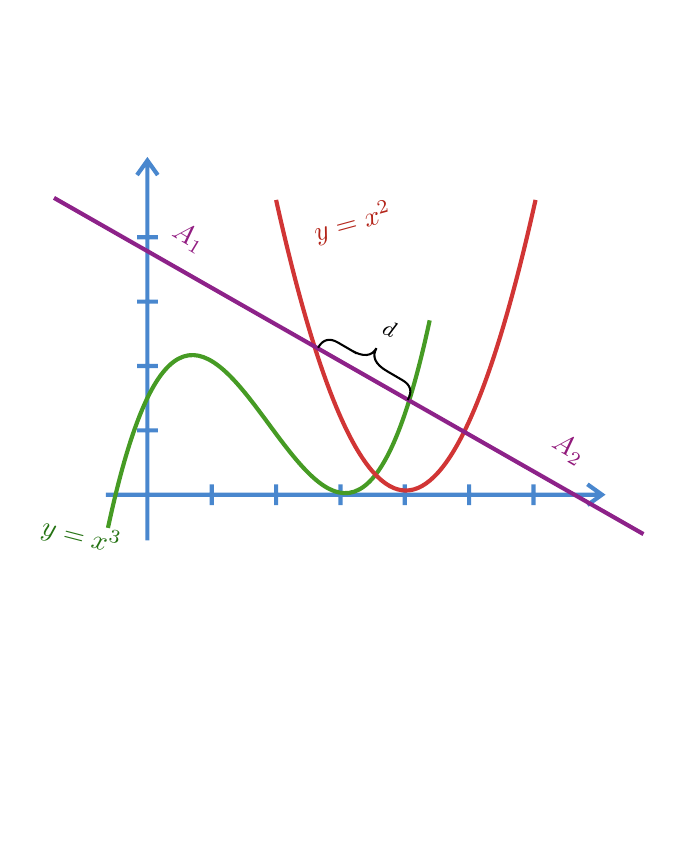
\begin{tikzpicture}[x=0.75pt,y=0.75pt,yscale=-1,xscale=1]
                            \draw [color={rgb, 255:red, 73; green, 135; blue, 206 }  ,draw opacity=1 ][line width=1.5]  (246,173) -- (485,173)(266,12) -- (266,195) (478,168) -- (485,173) -- (478,178) (261,19) -- (266,12) -- (271,19) (297,168) -- (297,178)(328,168) -- (328,178)(359,168) -- (359,178)(390,168) -- (390,178)(421,168) -- (421,178)(452,168) -- (452,178)(261,142) -- (271,142)(261,111) -- (271,111)(261,80) -- (271,80)(261,49) -- (271,49) ;
                            \draw   ;
                            \draw  [color={rgb, 255:red, 70; green, 155; blue, 36 }  ,draw opacity=1 ][line width=1.5]  (247,189) .. controls (298.67,-51) and (350.33,329) .. (402,89) ; 
                            \draw  [color={rgb, 255:red, 209; green, 53; blue, 53 }  ,draw opacity=1 ][line width=1.5]  (328,31) .. controls (369.67,217.67) and (411.33,217.67) .. (453,31) ;
                            \draw [color={rgb, 255:red, 141; green, 34; blue, 137 }  ,draw opacity=1 ][line width=1.5]    (221,30) -- (505,192) ;
                            \draw  [line width=0.75]  (391.4,127.4) .. controls (393.75,123.37) and (392.91,120.18) .. (388.88,117.83) -- (381.48,113.51) .. controls (375.72,110.15) and (374.02,106.45) .. (376.37,102.42) .. controls (374.02,106.45) and (369.96,106.79) .. (364.21,103.43)(366.8,104.94) -- (357.78,99.68) .. controls (353.75,97.33) and (350.55,98.17) .. (348.2,102.2) ;
                            \draw (286,49) node  [color={rgb, 255:red, 146; green, 29; blue, 130 }  ,opacity=1 ,rotate=-30.96]  {$A_{1}$};
                            \draw (469,151) node  [color={rgb, 255:red, 145; green, 25; blue, 123 }  ,opacity=1 ,rotate=-30.96]  {$A_{2}$};
                            \draw (234,193) node  [color={rgb, 255:red, 36; green, 114; blue, 18 }  ,opacity=1 ,rotate=-14.47]  {$y=x^{3}$};
                            \draw (365,42) node  [color={rgb, 255:red, 179; green, 35; blue, 24 }  ,opacity=1 ,rotate=-344.74]  {$y=x^{2}$};
                            \draw (382.8,93.2) node  [font=\footnotesize,rotate=-22.93]  {$d$};
                        \end{tikzpicture}
                    \end{center}
                \end{frame}

            \subsection{\texttt{tikz-cd}}
                \begin{frame}[fragile]{\texttt{tikz-cd}}
                    \begin{center}
                        \begin{tikzcd}[column sep=tiny]
                            & \pi_1(U_1) \ar[dr] \ar[drr, "j_1", bend left=20]
                            &
                            &[1.5em] \\
                            \pi_1(U_1\cap U_2) \ar[ur, "i_1"] \ar[dr, "i_2"']
                            &
                            & \pi_1(U_1) \ast_{ \pi_1(U_1\cap U_2)} \pi_1(U_2) \ar[r, dashed, "\simeq"]
                            & \pi_1(X) \\
                            & \pi_1(U_2) \ar[ur]\ar[urr, "j_2"', bend right=20]
                            &
                            &
                            \end{tikzcd}
                    \end{center}
                \end{frame}
            
            \subsection{\texttt{circuitikz}}
                \begin{frame}[fragile]{\texttt{circuitikz}}
                    \ctikzset{amplifiers/fill=cyan!15, resistors/fill=magenta!15}
                    \begin{circuitikz}[european]
                        \draw (0, 0) node[above]{$v_i$} to[short, o-] ++(1, 0) node[op amp, noinv input up, anchor=+](OA){\texttt{OA}} (OA.-) -- ++(0, -1) coordinate(FB) to[R=$R1$] ++(0, -2) node[ground]{} (FB) to[R=$R_2$, *-] (FB -| OA.out) -- (OA.out) to[short, *-o] ++(1, 0) node[above]{$v_o$}; 
                    \end{circuitikz}
                \end{frame}


    \section{Thanks to, I learn a lot from them!}
\end{document}